\subsection*{Anhang}\label{anhang}

\lstset{language=java}
\begin{lstlisting}[frame=htrbl, caption={Die Klasse 'SSHConstants.java'}, label={lst:SSHConstants}]
package app.sftp;

public class SSHConstants {
    public static String USERNAME = "";
    public static String PASSWORD = "";
}


\end{lstlisting}

\begin{figure}[h]
 \centering
 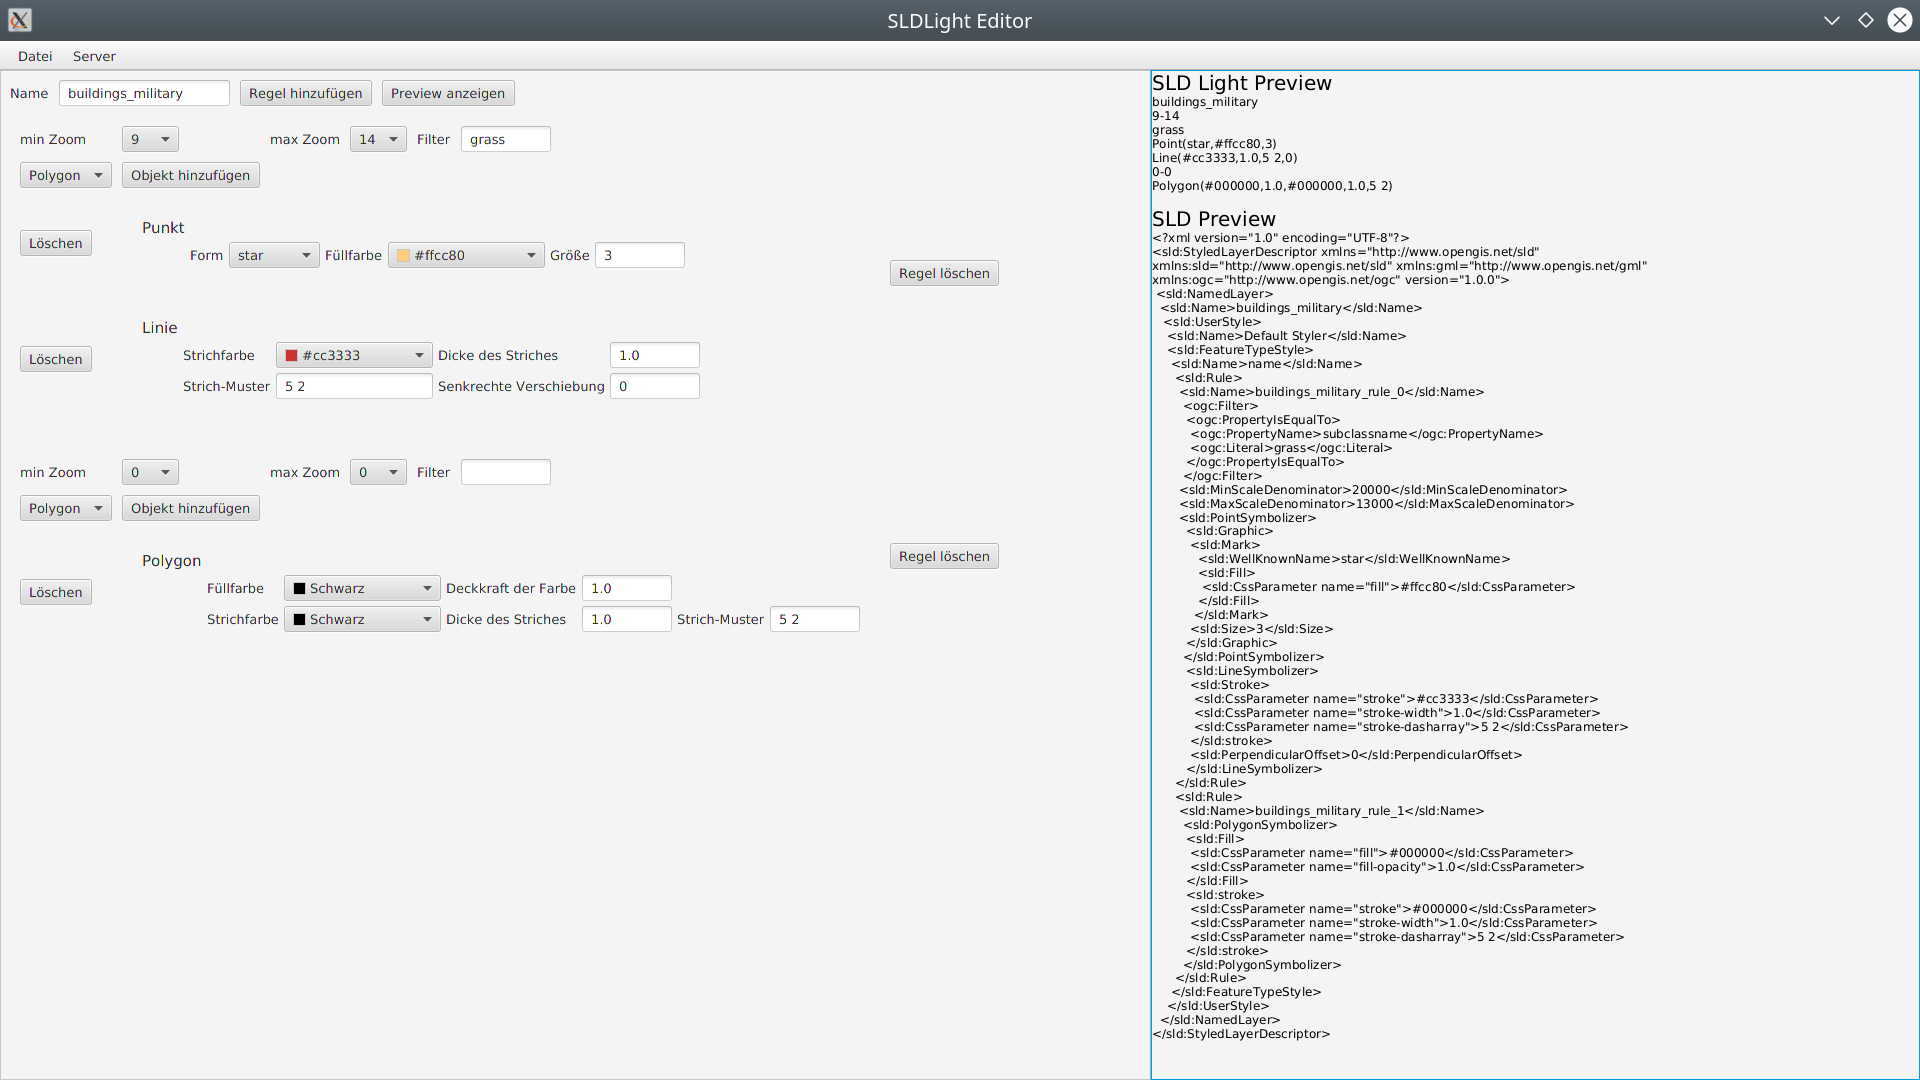
\includegraphics[width=1\textwidth]{abb/editor}
 \caption{Ansicht des Editors}\label{abb:editor}
\end{figure}

\lstset{language=java}
\begin{lstlisting}[frame=htrbl, caption={Beispiel für SLD-Light}, label={lst:SLDLight}]
buildings_military
9-14
grass
Point(star,#ffcc80,3)
Line(#cc3333,1.0,5 2,0)
0-0
Polygon(#000000,1.0,#000000,1.0,5 2)
\end{lstlisting}

\lstset{language=java}
\begin{lstlisting}[frame=htrbl, caption={Beispiel für SLD}, label={lst:SLD}]
<?xml version="1.0" encoding="UTF-8"?>
<sld:StyledLayerDescriptor xmlns="http://www.opengis.net/sld" xmlns:sld="http://www.opengis.net/sld" xmlns:gml="http://www.opengis.net/gml" xmlns:ogc="http://www.opengis.net/ogc" version="1.0.0">
 <sld:NamedLayer>
  <sld:Name>buildings_military</sld:Name>
   <sld:UserStyle>
    <sld:Name>Default Styler</sld:Name>
    <sld:FeatureTypeStyle>
     <sld:Name>name</sld:Name>
      <sld:Rule>
       <sld:Name>buildings_military_rule_0</sld:Name>
        <ogc:Filter>
         <ogc:PropertyIsEqualTo>
          <ogc:PropertyName>subclassname</ogc:PropertyName>
          <ogc:Literal>grass</ogc:Literal>
         </ogc:PropertyIsEqualTo>
        </ogc:Filter>
       <sld:MinScaleDenominator>20000</sld:MinScaleDenominator>
       <sld:MaxScaleDenominator>13000</sld:MaxScaleDenominator>
       <sld:PointSymbolizer>
         <sld:Graphic>
          <sld:Mark>
            <sld:WellKnownName>star</sld:WellKnownName>
            <sld:Fill>
             <sld:CssParameter name="fill">#ffcc80</sld:CssParameter>
            </sld:Fill>
           </sld:Mark>
          <sld:Size>3</sld:Size>
         </sld:Graphic>
        </sld:PointSymbolizer>
         <sld:LineSymbolizer>
          <sld:Stroke>
           <sld:CssParameter name="stroke">#cc3333</sld:CssParameter>
           <sld:CssParameter name="stroke-width">1.0</sld:CssParameter>
           <sld:CssParameter name="stroke-dasharray">5 2</sld:CssParameter>
          </sld:stroke>
          <sld:PerpendicularOffset>0</sld:PerpendicularOffset>
         </sld:LineSymbolizer>
      </sld:Rule>
      <sld:Rule>
       <sld:Name>buildings_military_rule_1</sld:Name>
        <sld:PolygonSymbolizer>
         <sld:Fill>
          <sld:CssParameter name="fill">#000000</sld:CssParameter>
          <sld:CssParameter name="fill-opacity">1.0</sld:CssParameter>
         </sld:Fill>
         <sld:stroke>
          <sld:CssParameter name="stroke">#000000</sld:CssParameter>
          <sld:CssParameter name="stroke-width">1.0</sld:CssParameter>
          <sld:CssParameter name="stroke-dasharray">5 2</sld:CssParameter>
         </sld:stroke>
        </sld:PolygonSymbolizer>
      </sld:Rule>
     </sld:FeatureTypeStyle>
    </sld:UserStyle>
  </sld:NamedLayer>
</sld:StyledLayerDescriptor>
\end{lstlisting}

\lstset{language=java}
\begin{lstlisting}[frame=htrbl, caption={Beispiel XML-Datei für Geoserver}, label={lst:XML_SLD}]
<style>
  <id>StyleInfoImpl-4e1160b8:160efbd149b:40ff</id>
  <name>buildings_military</name>
  <workspace>
    <id>WorkspaceInfoImpl-355a8844:15b19d1e2c3:-7ffe</id>
  </workspace>
  <format>sld</format>
  <languageVersion>
    <version>1.0.0</version>
  </languageVersion>
  <filename>buildings_military.sld</filename>
</style>
\end{lstlisting}

\begin{table}[h!]
  \begin{center}
    \begin{tabular}{ l | c }
	Zoomstufe & SLD-Wert \\
\hline
  0 & keine Angabe \\
  1 & 100000 \\
  2 & 80000 \\
  3 & 60000 \\
  4 & 50000 \\
  5 & 40000 \\
  6 & 30000 \\
  7 & 25000 \\
  8 & 22000 \\
  9 & 20000 \\
  10 & 18000 \\
  11 & 16000 \\
  12 & 15000 \\
  13 & 14000 \\
  14 & 13000 \\
  15 & 12000 \\
  16 & 8000 \\
	\end{tabular}
	
    \caption{Zoomstufen}
    \label{table:zoom}
  \end{center}
\end{table}
